% Shared standalone design for the editable figure reconstructions.
\documentclass[tikz,border=5pt,10pt]{standalone}
\usepackage[T1]{fontenc}
\usepackage[utf8]{inputenc}
\usepackage{newpxtext,newpxmath}
\usepackage[scaled=.94]{sourcesanspro}
\usepackage{pgfplots}
\pgfplotsset{compat=1.18}
\usetikzlibrary{arrows.meta,calc,positioning,decorations.pathreplacing,
  decorations.markings,patterns,matrix,shapes.geometric,fit,backgrounds,
  intersections,angles,quotes}
\definecolor{ink}{HTML}{203746}
\definecolor{accent}{HTML}{146C78}
\definecolor{muted}{HTML}{667780}
\definecolor{signalred}{HTML}{B94B44}
\color{ink}
\tikzset{>=Latex,line width=.8pt,
  every node/.style={font=\small},
  axis/.style={->,draw=muted,line width=.5pt},
  guide/.style={draw=muted,dashed,line width=.45pt},
  curve/.style={draw=accent,line width=1pt},
  marker/.style={circle,fill=accent,inner sep=1.5pt},
  labelbox/.style={fill=white,inner sep=2pt}}

\begin{document}
\begin{tikzpicture}[x=1.25cm,y=1.25cm]
\path[fill=accent!8](0,0)--(2.3,1.61)--(3.91,0)--cycle;
\path[fill=accent!25](0,0)--(2.3,1.61)--(2.3,0)--cycle;
\draw[axis](0,0)--(4.6,0)node[right]{$\lambda$};\draw[axis](0,0)--(0,4.4)node[above]{$\delta$};
\draw[ink] (0,3.91)--(3.91,0);\node[rotate=-45,above]at(1.2,2.71){$\delta+\lambda=T/K$};
\draw[accent](0,0)--(4.4,3.08)node[above]{$R\delta=S\lambda$};
\draw[guide](2.3,0)node[below]{$\lambda_{\max}$}--(2.3,1.61);\draw[ink,fill=white](2.3,1.61)circle(1.6pt);
\node at(1.65,.55){$\widetilde{\mathcal R}$};\node at(2.9,.55){$\mathcal R$};
\node[left]at(0,3.91){$T/K$};\node[below]at(3.91,0){$T/K$};
\node[anchor=west,align=left]at(5.0,2.8){$\mathcal R:\quad\delta+\lambda<T/K,$\\[5pt]$\phantom{\mathcal R:\quad}R\delta<S\lambda$\\[12pt]$\widetilde{\mathcal R}:\quad\delta/\lambda<S/R,$\\[5pt]$\phantom{\widetilde{\mathcal R}:\quad}0<\lambda<\lambda_{\max}$\\[12pt]$\lambda_{\max}=\dfrac{TR}{K(R+S)}$};
\node[anchor=west,align=left,text width=4.6cm,font=\footnotesize]at(5.0,.25){$\delta\geq0$; the oblique boundaries are excluded.};
\end{tikzpicture}
\end{document}
